
{\setbeamertemplate{footline}{}
\begin{frame}[noframenumbering]
		\titlepage
\end{frame}
}

\begin{frame}{Язык Java в физике}
	Язык Java используется для создания сложных многопоточных приложений, в том
	числе для физических исследований в ЦЕРНе: 
	\begin{enumerate}
		\item Системы управления Большим Адронным Коллайдером.
		\item Многопоточная обработка экспериментальных данных: Colt Parallel. 
	\end{enumerate}
\end{frame}

\begin{frame}{Недостатки потоков}
	\begin{enumerate}
		\item Создание потока дорогостоящая операция в ОС.
		\item Переключение потоков несет в себе серьезные накладные расходы.
	\end{enumerate}
	Существует альтернативный способ организации параллельных систем -- \textbf{сопрограммы}. 
\end{frame}

\begin{frame}{Сопрограммы}
	\begin{itemize}
		\item \textbf{Сопрограмма} (англ. coroutine) - программный модуль, организованный для обеспечения взаимодействия с другими модулями по принципу кооперативной многозадачности.
		
		\item Сопрограммы способны приостанавливать свое выполнение, сохраняя \textit{контекст} 
		(программный стек и регистры), и передавать управление другой.
	\end{itemize}
\end{frame}

\begin{frame}{Реализация в языках программирования}
	\begin{figure}
	\centering
	\hfill
	\begin{subfigure}[b]{0.22\linewidth}
		
\includegraphics[width=\linewidth]{images/cpp.png}
		\caption{С++20}
	\end{subfigure}
	\hfill
	\begin{subfigure}[b]{0.25\linewidth}
		
\includegraphics[width=\linewidth]{images/csharp.jpg} 
		\caption{С\#}
	\end{subfigure}
	\hfill
	\begin{subfigure}[b]{0.27\linewidth}
		
\includegraphics[width=\linewidth]{images/go.jpg}
		\caption{Go}
	\end{subfigure}
	
	\end{figure}
	\par
	В языке Java сопрограммы не реализованы.
\end{frame}

\begin{frame}
	
\includegraphics[scale=0.4]{images/loom.jpg}
	\begin{itemize}
		\item Project Loom – проект на базе OpenJDK, целью которого является разработка сопрограмм для языка Java. 
		\item На данный момент уже доступна ранняя версия проекта.
	\end{itemize}
\end{frame}

\begin{frame}{Цели и задачи}
	Цель: изучить применимость сопрограмм вместо потоков в программах Java.
	\par
	Поставленные задачи:
	\begin{itemize}
		\item Разработать тесты для сравнения производительности потоков и сопрограмм.
		\item Реализовать модуль сопрограмм.
		\item Сравнить производительность сопрограмм и потоков.
		\item Выявить ключевые плюсы использования сопрограмм.
	\end{itemize}
	Работа проводится на базе Huawei JDK.
\end{frame} 

\begin{frame}{Тесты производительности}
	Был создан набор тестов производительности сопрограмм для языков Go, Java (с “Loom Project”).
	
	Тесты создавались для измерения 3 параметров.
	\begin{itemize}
		\item Время создания потока/сопрограммы. 
		\item Скорость переключения контекста.
		\item Потребление памяти.
	\end{itemize}
	Репозиторий с тестами: https://github.com/minium2/coroutines-benchmark
\end{frame}

\begin{frame}{Переключение сопрограмм}
	\begin{figure}
		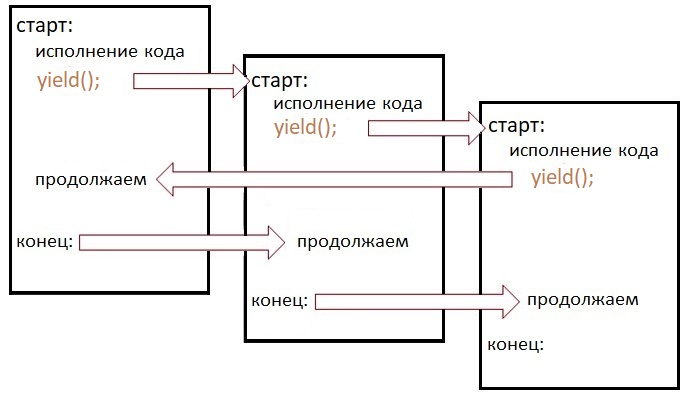
\includegraphics[scale=0.5]{images/scheme.jpg}
	\end{figure}
	\par
	\begin{itemize}
		\item Функция yeild() переключает управление от одной сопрограммы другой.
		\item Завершение выполнения сопрограммы приводит к переключению на другую.
	\end{itemize}
\end{frame}

\begin{frame}{Подходы к реализации переключения сопрограмм}
	\begin{itemize}
		\item OpenJDK/"Loom": копирование стека сопрограммы при переключении.
		\item Go: изменение указателя стека.
	\end{itemize}

	В HuaweiJDK выбран подход языка Go, поскольку он более эффективен.
\end{frame}

\begin{frame}{Измерение скорости переключения сопрограмм в управляемых средах}
	Ubuntu, kernel 4.15, Intel Core i7-8700, 4.6 ГГц, 32 Гб ОЗУ
	\par Каждое значение усреднено по 100 измерениям. 
	
	\begin{table}[H]
		%\caption{Число переключений корутин}\label{inc-matrix}
		\textit{\begin{tabular}{|c|c|c|c|c|c|}
				\hline \multirow{2}{*}{Шт.} & \multicolumn{3}{|c|}{Число переключений, тыс./сек.}                  \\
				\cline{2-4}               & HuaweiJDK                  & OpenJDK/"Loom"     & Go                   \\
				\hline 100                & \numprint{12980} $\pm$ 540 & \numprint{1900} $\pm$ 20\phantom{0}    & \numprint{18187} $\pm$ 219 \\
				\hline \numprint{1000}    & \numprint{11420} $\pm$ 694 & \numprint{1775} $\pm$ 20\phantom{0}    & \numprint{17934} $\pm$ 332 \\
				\hline \numprint{5000}    & \phantom{0}\numprint{5875} $\pm$ 183   & \numprint{1703} $\pm$ 30\phantom{0}    & \numprint{12892} $\pm$ 339 \\  
				\hline \numprint{10000}   & \phantom{0}\numprint{4459} $\pm$ 162 & \numprint{1924} $\pm$ 235  & \numprint{8307} $\pm$ 80   \\  
				\hline \numprint{20000}   & \numprint{3604} $\pm$ 93 & \numprint{1863} $\pm$ 217   			  & \numprint{7045} $\pm$ 72   \\ 
				\hline \numprint{30000}   & \numprint{3031} $\pm$ 94 & \numprint{1772} $\pm$ 182   			  & \numprint{6391} $\pm$ 94   \\ 
				\hline \numprint{40000}   & \numprint{2653} $\pm$ 87 & \numprint{1606} $\pm$ 194              & \numprint{5790} $\pm$ 67   \\ 
				\hline \numprint{50000}   & \numprint{2315} $\pm$ 60 & \numprint{1503} $\pm$ 157              & \phantom{0}\numprint{5292} $\pm$ 122  \\  
				\hline 
		\end{tabular}}
	\end{table}	
\end{frame}

\begin{frame}{Измерение скорости переключения потоков и сопрограмм}
	Ubuntu, kernel 4.15, Intel Core i7-8700, 4.6 ГГц, 32 Гб ОЗУ, HuaweiJDK
	\par Каждое значение усреднено по 100 измерениям. 
	\par Для измерения используется только одно ядро ЦП.
	\begin{table}[H]
		%\caption{Число переключений корутин}\label{inc-matrix}
		\textit{\begin{tabular}{|c|c|c|c|c|c|}
				\hline \multirow{2}{*}{Шт.} & \multicolumn{2}{|c|}{Число переключений, тыс./сек.} \\
				\cline{2-3}              & Сопрограммы                           & Потоки                    \\
				\hline 100               & \numprint{12980} $\pm$ 540            & \numprint{2306} $\pm$ 50  \\
				\hline \numprint{1000}   & \numprint{11420} $\pm$ 694            & \numprint{2300} $\pm$ 27  \\
				\hline \numprint{5000}   & \phantom{0}\numprint{5875} $\pm$ 183  & \numprint{1554} $\pm$ 37   \\
				\hline \numprint{10000}  & \phantom{0}\numprint{4459} $\pm$ 162  & \numprint{1016} $\pm$ 29   \\ 
				\hline \numprint{20000}  & \numprint{3604} $\pm$ 93              & \phantom{0}753   $\pm$ 28              \\ 
				\hline \numprint{30000}  & \numprint{3031} $\pm$ 94              & \phantom{0}556   $\pm$ 16              \\ 
				\hline \numprint{40000}  & \numprint{2653} $\pm$ 87              & \phantom{0}436   $\pm$ 12              \\ 
				\hline \numprint{50000}  & \numprint{2315} $\pm$ 60              & 		      361   $\pm$ 8               \\ 
				\hline 
			\end{tabular}
		}
	\end{table}
\end{frame}

\begin{frame}{Измерение потребление памяти сопрограмм в управляемых средах}
	Ubuntu, kernel 4.15, Intel Core i7-8700, 4.6 ГГц, 32 Гб ОЗУ
	\begin{table}[H]
		\textit{\begin{tabular}{|c|c|c|c|c|c|}
			\hline \multirow{2}{*}{Шт.} & \multicolumn{3}{|c|}{Резидентная память}  \\
			\cline{2-4}    & HuaweiJDK   & OpenJDK/"Loom"    & Go        \\
			\hline 100     & 18 Mб       & 130 Mб    		 & 3,040 Mб  \\
			\hline 1000    & 22 Mб       & 161 Mб     		 & 3,105 Mб  \\
			\hline 5000    & 32 Mб       & 187 Mб    		 & 3,156 Mб  \\
			\hline 10000   & 37 Mб       & 193 Mб     		 & 3,308 Mб  \\
			\hline 20000   & 45 Mб       & 196 Mб     		 & 3,320 Mб  \\
			\hline 30000   & 49 Mб       & 197 Mб     		 & 3,350 Mб  \\
			\hline 40000   & 51 Mб       & 200 Mб    		 & 3,390 Mб  \\
			\hline 50000   & 57 Mб       & 202 Mб    		 & 3,407 Mб  \\ 
			\hline 
		\end{tabular}}
	\end{table}
\end{frame}

\begin{frame}{Измерение потребление памяти потоков}
	Ubuntu, kernel 4.15, Intel Core i7-8700, 4.6 ГГц, 32 Гб ОЗУ, HuaweiJDK
	\begin{table}[H]
		%\caption{Число переключений корутин}\label{inc-matrix}
		\textit{\begin{tabular}{|c|c|c|c|c|c|}
			\hline \multirow{2}{*}{Шт.} & \multicolumn{2}{|c|}{Размер физической памяти}  \\
			\cline{2-3}    & Сопрограммы   & Потоки    \\
			\hline 100     & 18 Mб         & 34 Mб     \\
			\hline 1000    & 22 Mб         & 35 Mб     \\
			\hline 5000    & 32 Mб         & 37 Mб     \\
			\hline 10000   & 37 Mб         & 40 Mб     \\
			\hline 20000   & 45 Mб         & 49 Mб     \\
			\hline 30000   & 49 Mб         & 56 Mб     \\
			\hline 40000   & 51 Mб         & 63 Mб     \\
			\hline 50000   & 57 Mб         & 72 Mб     \\ 
			\hline 
		\end{tabular}}
	\end{table}
\end{frame}

\begin{frame}{Ключевые отличия от потоков ОС}
	\begin{itemize}
		\item Переключение контекста сопрограммы требует меньше накладных расходов, чем переключение потока.
		\item Как правило меньший размер стека, а значит, потребление памяти так же меньше.
	\end{itemize}
\end{frame}

\begin{frame}{План дальнейших работ} 
	\begin{itemize}
		\item Поддержать synchronized блоков.
		\item Реализовать переключение сопрограммы при вызове ввода--вывода.
		\item Оценить возможный рост производительности от применения сопрограмм в промышленных
		проектах (например в Colt Parallel).
	\end{itemize}
\end{frame}

\begin{frame}{Результаты}
	\begin{itemize}
		\item Создан набор тестов для сравнения производительности потоков и сопрограмм.
		\item Реализован базовый прототип сопрограмм на базе HuaweiJDK.
		\item Проведен анализ результатов тестов производительности.
		\item Выявлены ключевые отличия сопрограмм от потоков.
	\end{itemize}
\end{frame}

